\documentclass{report}


\usepackage{graphicx}

\usepackage{amsmath}
\usepackage{graphicx}
\usepackage{ulem}
\usepackage{float}
\usepackage[utf8]{inputenc}
\usepackage{gensymb}
\usepackage{amsmath}
\usepackage{amssymb}
\usepackage{mathtools}
\newcommand{\partder}[1]{\frac{\partial h^l}{\partial #1}}

\graphicspath{{figures/}}

\title{OCS Hints for Questions}
\author{Julian Wolf}
\begin{document}
\maketitle
%%%%%%%%%%%%%%%%%%%%%%%%%%%%%%%%%%%%%%%%%%%%%%%%%%%%%%%%%%%%%%%%%%
\section*{Derivations}
Die Antworten sind teilweise unvollständig, einerseits, weil er die Antworten als "Eh Klar" abgestempelt hat, anderer seits weil er so schnell durchging, dass ein Mitschreiben nicht mehr möglich war. 

\begin{enumerate}
%%%%%%%%%%%%%%%%%%%%%%%%%%%%%%%%%%%%%%%%%%%%%%%%%%%%%%%%%%%
\item Draw level lines and arrows
\begin{itemize}
\item objective function is the function we want to minimize
\item constraint set is a set of functions
\item optimal solution: find $f(x^*) \leq f(x), \forall x \in X$
\item level set: compareable to level lines of terrain, convex function $=>$ convex level set (but there are non convex fct with convex level sets), 
\end{itemize}

%%%%%%%%%%%%%%%%%%%%%%%%%%%%%%%%%%%%%%%%%%%%%%%%%%%%%%%%%%%
\item 
\begin{itemize}
\item \textbf{Linear}: Objective Function and Constraints may only be linear
$min\ c^Tx, s.t.\ Ax \leq b, x \geq 0$\\
Polynomial solvable
\item \textbf{Non Linear}: Objective Function and Constriants may  be non linear
$min\ \frac{1}{2} x^TQx + c^Tx, s.t.\ Ax \leq b, Ex = d$\\
Q symmetrical and pos. definite, polynomial solvable
\item \textbf{Quadratic}: objective function is quadratic, constraints are linear	
$min_{x \in \mathbb{R}}\ f_0(x) \texttt{ (objective)},$\\
$s.t.\ f_i(x) \leq i=0..m \texttt{ (contraints)}$\\
polynomial time
\item \textbf{convex set}: 
$\alpha x + (1 - \alpha)y \ in X, \forall x, y \in X, \alpha \in [0, 1]$
\item \textbf{convex fct}:
$f(\alpha x + (1 - \alpha)y) \leq \alpha f(x) + (1 - \alpha)f(y) , \forall x, y \in X, \alpha \in [0, 1]$ 
\end{itemize}
%%%%%%%%%%%%%%%%%%%%%%%%%%%%%%%%%%%%%%%%%%%%%%%%%%%%%%%%%%%
\item 
\begin{itemize}
	\item When hessian is strictly positive, it is a strict global maximum
	\item \textbf{unconst Local minimum:} $f(x^*) \leq f(x), \forall x \texttt{ with } || x - x^* || \leq \varepsilon$
	\item \textbf{unconst global minimum:} $f(x^*) \leq f(x), \forall x \in \mathbb{R}$
\end{itemize}

\begin{figure}[H]
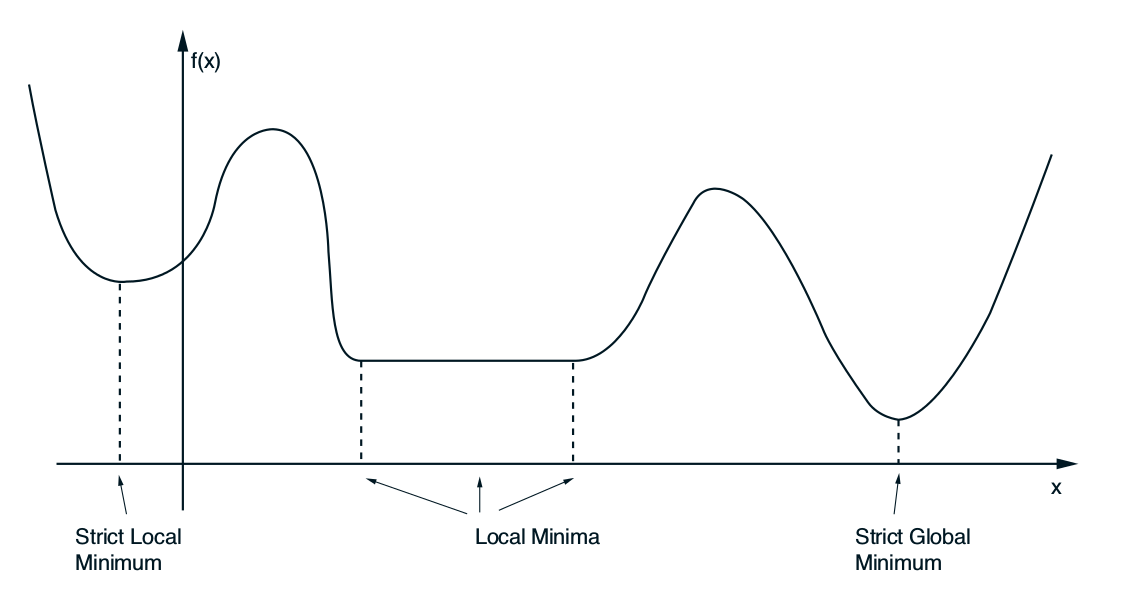
\includegraphics[width=\textwidth]{loc_glob_min.png}
\caption{Local/Global minimas\label{fig:min}}
\end{figure}	
%%%%%%%%%%%%%%%%%%%%%%%%%%%%%%%%%%%%%%%%%%%%%%%%%%%%%%%%%%%
\item 
\begin{itemize}
\item If positive and negative Eigenvalues, we can not define convexity
\item First order necessessary optimality condition: $\nabla f(x^*) = 0$
\item Second order necessessary optimality condition: $\nabla^2 f(x^*) $ is positive semi definite

\begin{figure}[H]
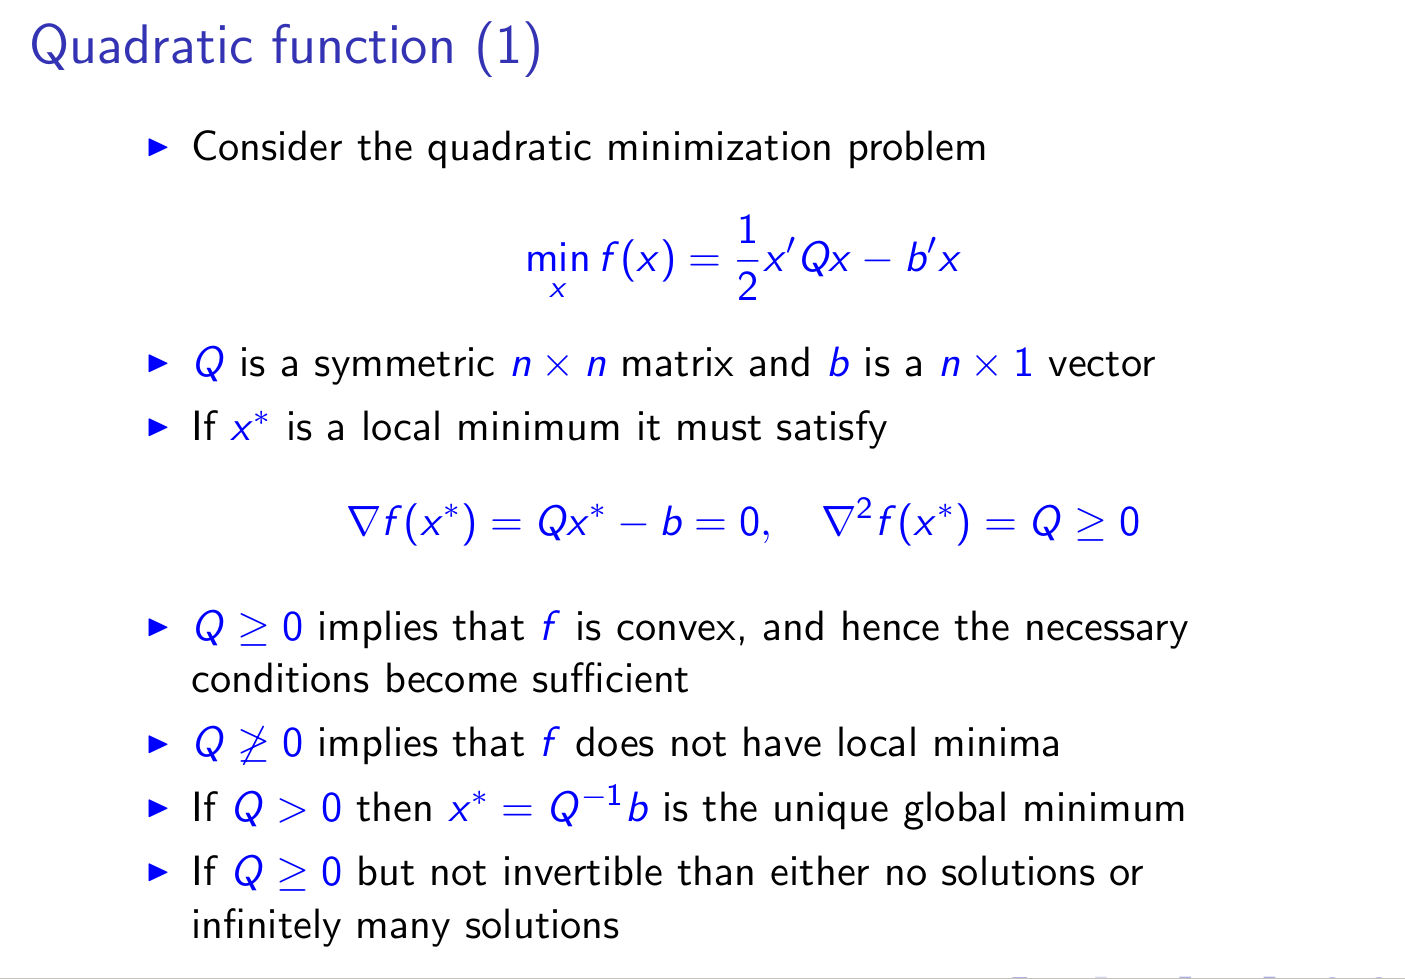
\includegraphics[width=\textwidth]{cond_quad_q.png}
\caption{Different scenarios for Q\label{fig:cond_quad}}
\end{figure}	
\end{itemize}

%%%%%%%%%%%%%%%%%%%%%%%%%%%%%%%%%%%%%%%%%%%%%%%%%%%%%%%%%%%
\item 
\begin{itemize}
\item Descent direction: angle of step and derivation direction $< 90^\circ$
\item General form of gradient method: \\
1. Choose an initial vector $x ^0 \in \mathbb{R}^n$\\
2. Choose a descent direction $d^k$ that satisfies $\nabla f (x^k)'  d^k < 0$\\
3. Choose a positive step size $\alpha^k$\\
4. Compute the new vector as\\
$x^{k+1} = x^k + \alpha^k d^k$\\
5. Set $k = k + 1$ and goto 2
\begin{figure}[H]
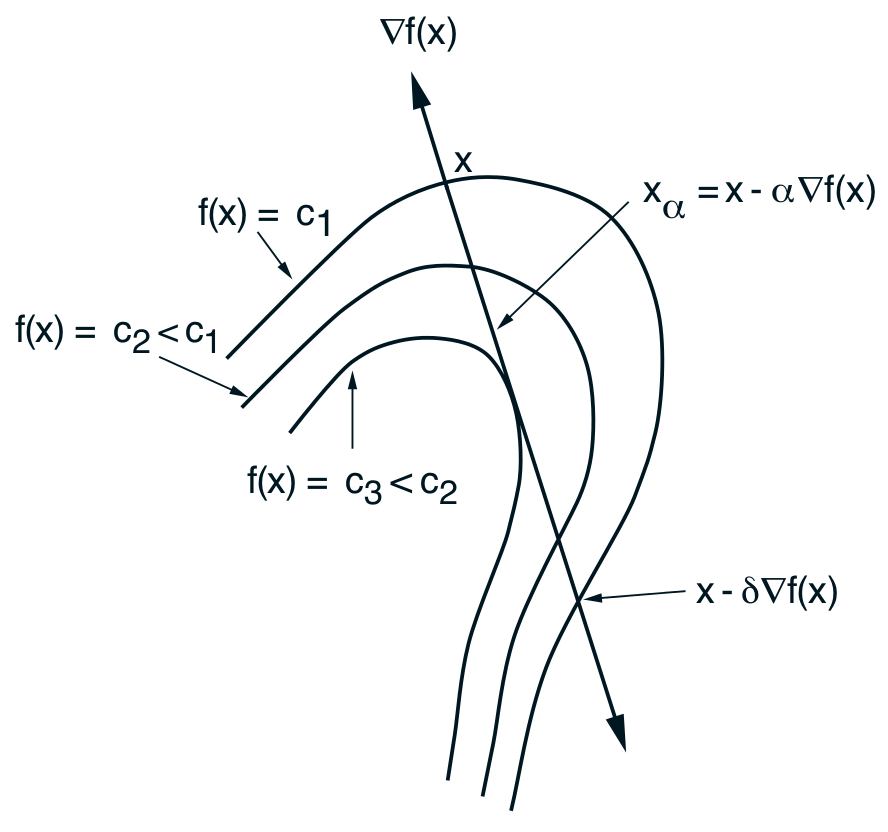
\includegraphics[width=\textwidth]{desc_dir.png}
\caption{Simple descent direction\label{fig:desc_dir}}
\end{figure}
\end{itemize}

%%%%%%%%%%%%%%%%%%%%%%%%%%%%%%%%%%%%%%%%%%%%%%%%%%%%%%%%%%%
\item $d^k = -D^k \nabla f (x^k )$
\begin{itemize}
	\item Identity: $D^k = I$, = Gradient descent, zig zagging problem, very bad on Rosenbrock Fct
	\item Hessian: $D^k = \nabla^2 f(x^k)$, = Newtons method, very fast convergence, very good on rosenbrock, unstable in despite of initial values (may diverge or find local maxima instead of minima), con: calculation of inverse of hessian - very expensive in large networks
	\item Diagonal Hessian (approximation of Newton): $d_i^k \approx \left(
\frac{\partial^2  f (x^k)}{(\partial x_i)^2}
\right)^{-1}$, very bad performance on Rosenbrock, 
	\item Gauss Newton method: Too complicated to remember, replace $D^k$ with non linear least square problem, even better performance on rosenbrock then newton, con: again calculation of inverse, but not of hessian
	\item \textbf{Step size} $\alpha$: 
	\begin{itemize}
		\item \textbf{Minimization rule:} choose $\alpha$ such that $f(x + \alpha d)$ is minimized along $d$. Hard if $f$ is complicated
		\item \textbf{Limited minimization rule:} iterative: start small and increase size of $\alpha$ until $f(x)$ is bigger then before, then choose the previous. Easy to implement
		\item \textbf{Armijo rule:} it is not sufficient that $f(x^{k+1}) < f(x^k)$, thus, the step sizes $\beta^ms$ for $m = 0,1,...$ are chosen such that the energy decrease is sufficiently large (dependent on derivation of $f(x)$, formula too complicated), or graphical:
	\begin{figure}[H]
	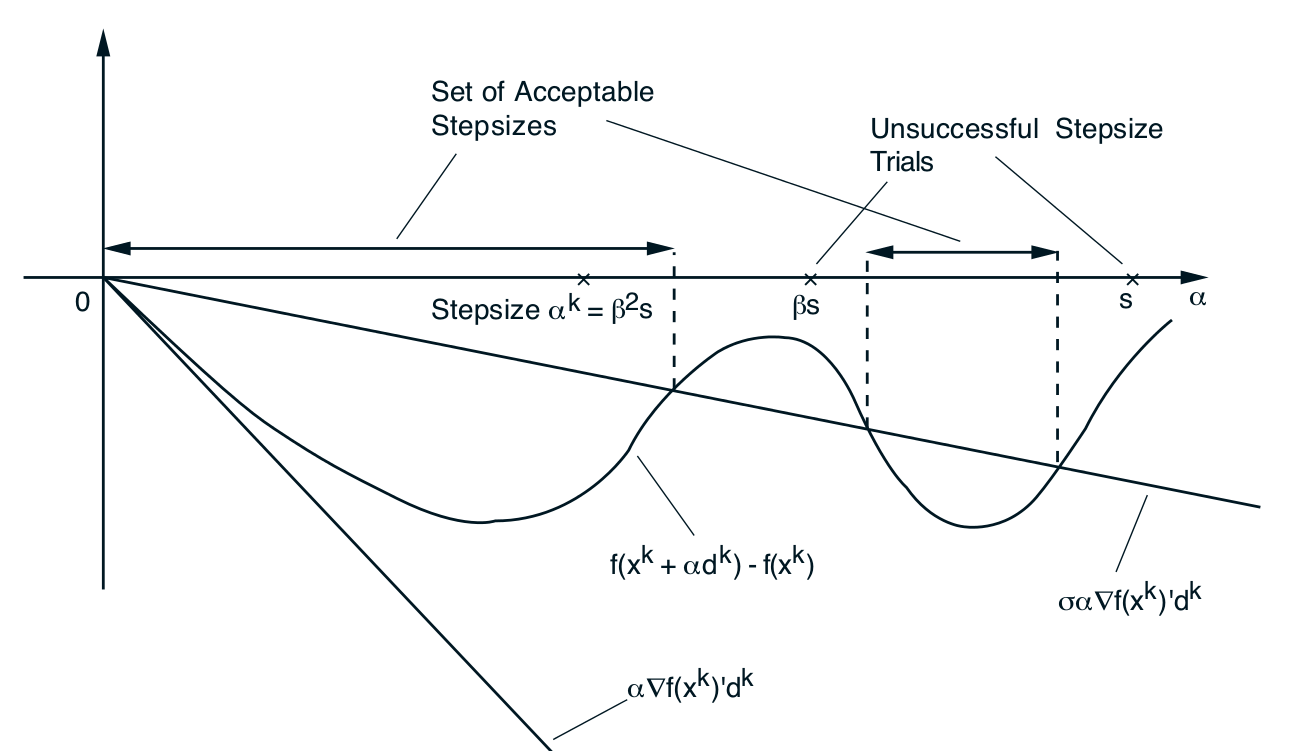
\includegraphics[width=\textwidth]{armijo.png}
	\caption{Graphical representation of the idea of Armijo\label{fig:desc_dir}}
	\end{figure}
		
	\end{itemize}
\end{itemize}

%%%%%%%%%%%%%%%%%%%%%%%%%%%%%%%%%%%%%%%%%%%%%%%%%%%%%%%%%%%
\item \begin{itemize}

	\item  there exists a definite real number such that, for every pair of points on the graph of this function, the absolute value of the slope of the line connecting them is not greater than this real number
	
	\item (There is something missing here)
	
\end{itemize}

%%%%%%%%%%%%%%%%%%%%%%%%%%%%%%%%%%%%%%%%%%%%%%%%%%%%%%%%%%%
\item 
\begin{itemize}
	\item \textbf{Linear:} $\limsup_{k \rightarrow \infty} \frac{e(x^{k+1})}{e(x^k)}\leq \beta$ (blue line)
	\item \textbf{superlinear:} $\limsup_{k \rightarrow \infty} \frac{e(x^{k+1})}{e(x^k)^p} < \infty$ (red line)
	\item \textbf{sublinear:} $\limsup_{k \rightarrow \infty} \frac{e(x^{k+1})}{e(x^k)} = 1$ (black line)
\end{itemize}

\begin{figure}[H]
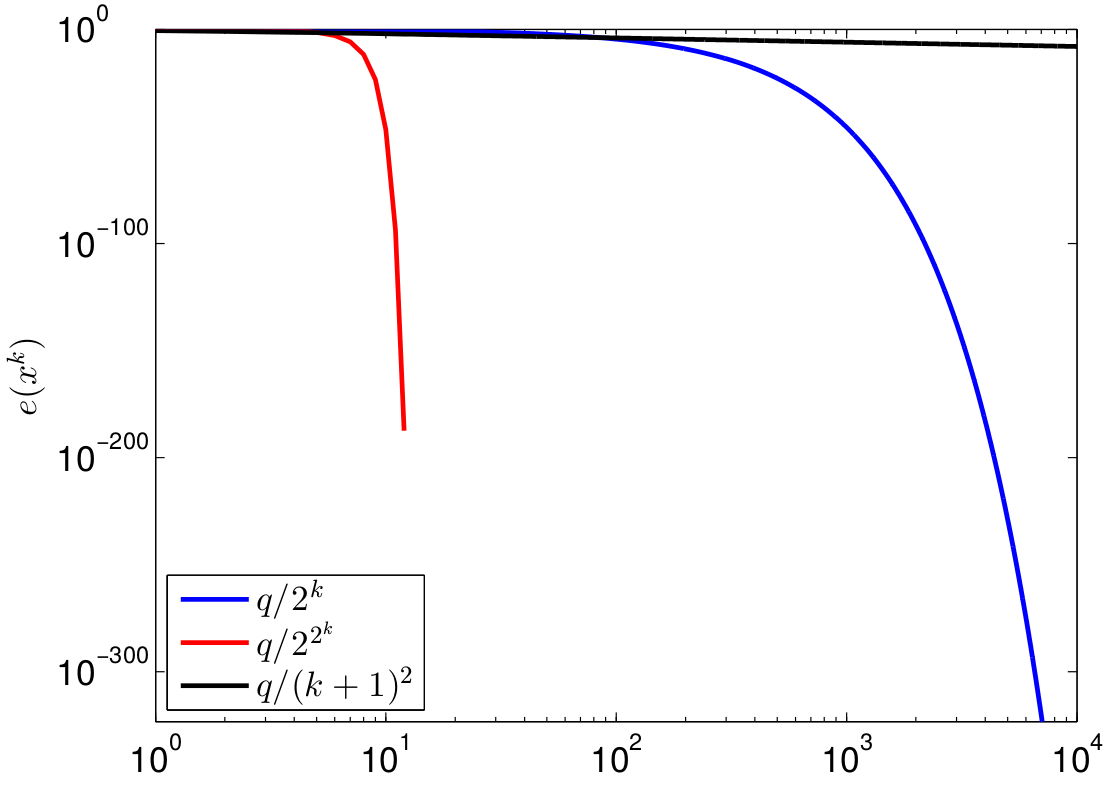
\includegraphics[width=10cm]{convergence.png}
\caption{Graphical representation of linear, superinear and sublinear convergence \label{fig:desc_dir}}
\end{figure}

%%%%%%%%%%%%%%%%%%%%%%%%%%%%%%%%%%%%%%%%%%%%%%%%%%%%%%%%%%%
\item \begin{itemize}
	\item $\tilde{g}(x, x^k) = g(x^k) + \nabla g(x^k)'(x - x^k)$
	\item is affine: because the derivation of the function is independent to a move of constants?!?!?
\end{itemize}
%%%%%%%%%%%%%%%%%%%%%%%%%%%%%%%%%%%%%%%%%%%%%%%%%%%%%%%%%%%
\item \textbf{Linear}:
\begin{itemize}
	\item pointcloud, best fitting by polynomial equations
	\item Solve least square problem to find optimal parameters
	\item $\frac{1}{2}|| Ax - z ||^2$
\end{itemize} 
\textbf{Non-Linear:}
\begin{itemize}
	\item Measure distance to beacons to get our own unkown location
	\item non linear least squares problem
	\item $min_x \frac{1}{2} \sum_{i = 1^m} (d_i - \sqrt{(x_i - p_1^i)^2 + (x_2 - p_2^i)^2})^2$
\end{itemize} 
\textbf{Gauss-Newton}:
\begin{itemize}
	\item Uses $(\nabla g(x^k)\nabla g(x^k)')^{-1}$ instead of hessian
	\item Approximates Current point with parabola and minimizes this subproblem (as plain Newton)
\end{itemize}
(check this shit out)
%%%%%%%%%%%%%%%%%%%%%%%%%%%%%%%%%%%%%%%%%%%%%%%%%%%%%%%%%%%
\item \begin{itemize}
	\item incremental of gauss newton - incremental growing least squares estimate
	\item example watertank: many measurements with noise - a very good and fast convergence to correct level is reached
	\item extended Kalman Filter: input data behaves according to a function
\end{itemize}

%%%%%%%%%%%%%%%%%%%%%%%%%%%%%%%%%%%%%%%%%%%%%%%%%%%%%%%%%%%
\item \begin{itemize}
	\item $Q$ positive definite: $\left(\frac{\sqrt{L/I}-1}{\sqrt{L/I} + 1}\right)^n || x^0  - x* ||$
	\item $Q$ positive semidefinite: not motivated to write formula
	\item Best method: conjugate gradient method (by Polyak) see next question
\end{itemize}
%%%%%%%%%%%%%%%%%%%%%%%%%%%%%%%%%%%%%%%%%%%%%%%%%%%%%%%%%%%
\item \begin{itemize}
	\item Motivation: converge faster the GD but avoid Newton overhead
	\item Q-conjugate if: $d^i  Q d^j = 0, \forall i, j \texttt{ with } i \neq j$
	\item Algorithm: 
	Use Gram-Schmidt to find conjugate direction, calculate new search direction (easy as all but one coefficient are zero), choose $\alpha^k$ by minimization method, algorithm terminates after at most n steps. 
\end{itemize}
(I think this is the algorithm where every single dimension is differenciated and optimized - hence the n termination)
%%%%%%%%%%%%%%%%%%%%%%%%%%%%%%%%%%%%%%%%%%%%%%%%%%%%%%%%%%%
\item \begin{itemize}
	\item Heavy-ball: Idea is like in physics: a ball uses its momentum it gained beforehand to overcome small increases or flat areas of its way
	\item Problem: function needs to be strongly $\mu > 0$ convex and twice continously differentiable
	\item Nesterov overcomes the twice diff. and the $\mu > 0$ problem by a dynamic choice of overrelaxation param $\beta^k = \frac{t_k - 1}{t_k + 1} \rightarrow 1$, gradient is evaluated at extrapolated point
	\item Both algorithms are optimal
	\item HB is optimal like the $Q$ positive semidefinite optimality, Nesterov also yields linear convergence rate on strongly convex sets
	\end{itemize}
%%%%%%%%%%%%%%%%%%%%%%%%%%%%%%%%%%%%%%%%%%%%%%%%%%%%%%%%%%%
\item \begin{itemize}
	\item the gradient $\nabla f(x^*)$ makes an angle $\leq$ 90 in all feasable points
	\item this condition is in general not reachable

\end{itemize}
\begin{figure}[H]
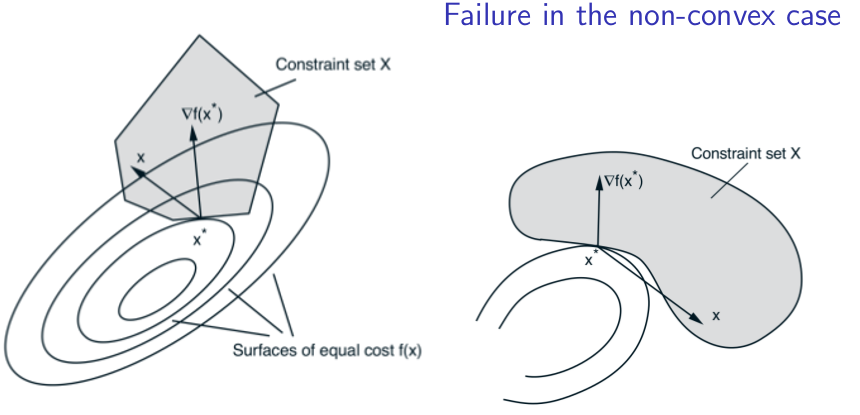
\includegraphics[width=\textwidth]{non_convex.png}
\caption{Graphical representation of convex and non-convex set \label{fig:convex}}
\end{figure}
%%%%%%%%%%%%%%%%%%%%%%%%%%%%%%%%%%%%%%%%%%%%%%%%%%%%%%%%%%%
\item First pages of slide 10
%%%%%%%%%%%%%%%%%%%%%%%%%%%%%%%%%%%%%%%%%%%%%%%%%%%%%%%%%%%
\item middle/end of pages slide 10 - start in interior and just take small steps $->$ we can ignore constraint under these conditions
%%%%%%%%%%%%%%%%%%%%%%%%%%%%%%%%%%%%%%%%%%%%%%%%%%%%%%%%%%%
\item \sout{too fast}
%%%%%%%%%%%%%%%%%%%%%%%%%%%%%%%%%%%%%%%%%%%%%%%%%%%%%%%%%%%
\item see figure~\ref{fig:ex1}

%%%%%%%%%%%%%%%%%%%%%%%%%%%%%%%%%%%%%%%%%%%%%%%%%%%%%%%%%%%
\item see figure~\ref{fig:ex2}

%%%%%%%%%%%%%%%%%%%%%%%%%%%%%%%%%%%%%%%%%%%%%%%%%%%%%%%%%%%
\item see figure~\ref{fig:ex2}


\end{enumerate}
\begin{figure}[H]
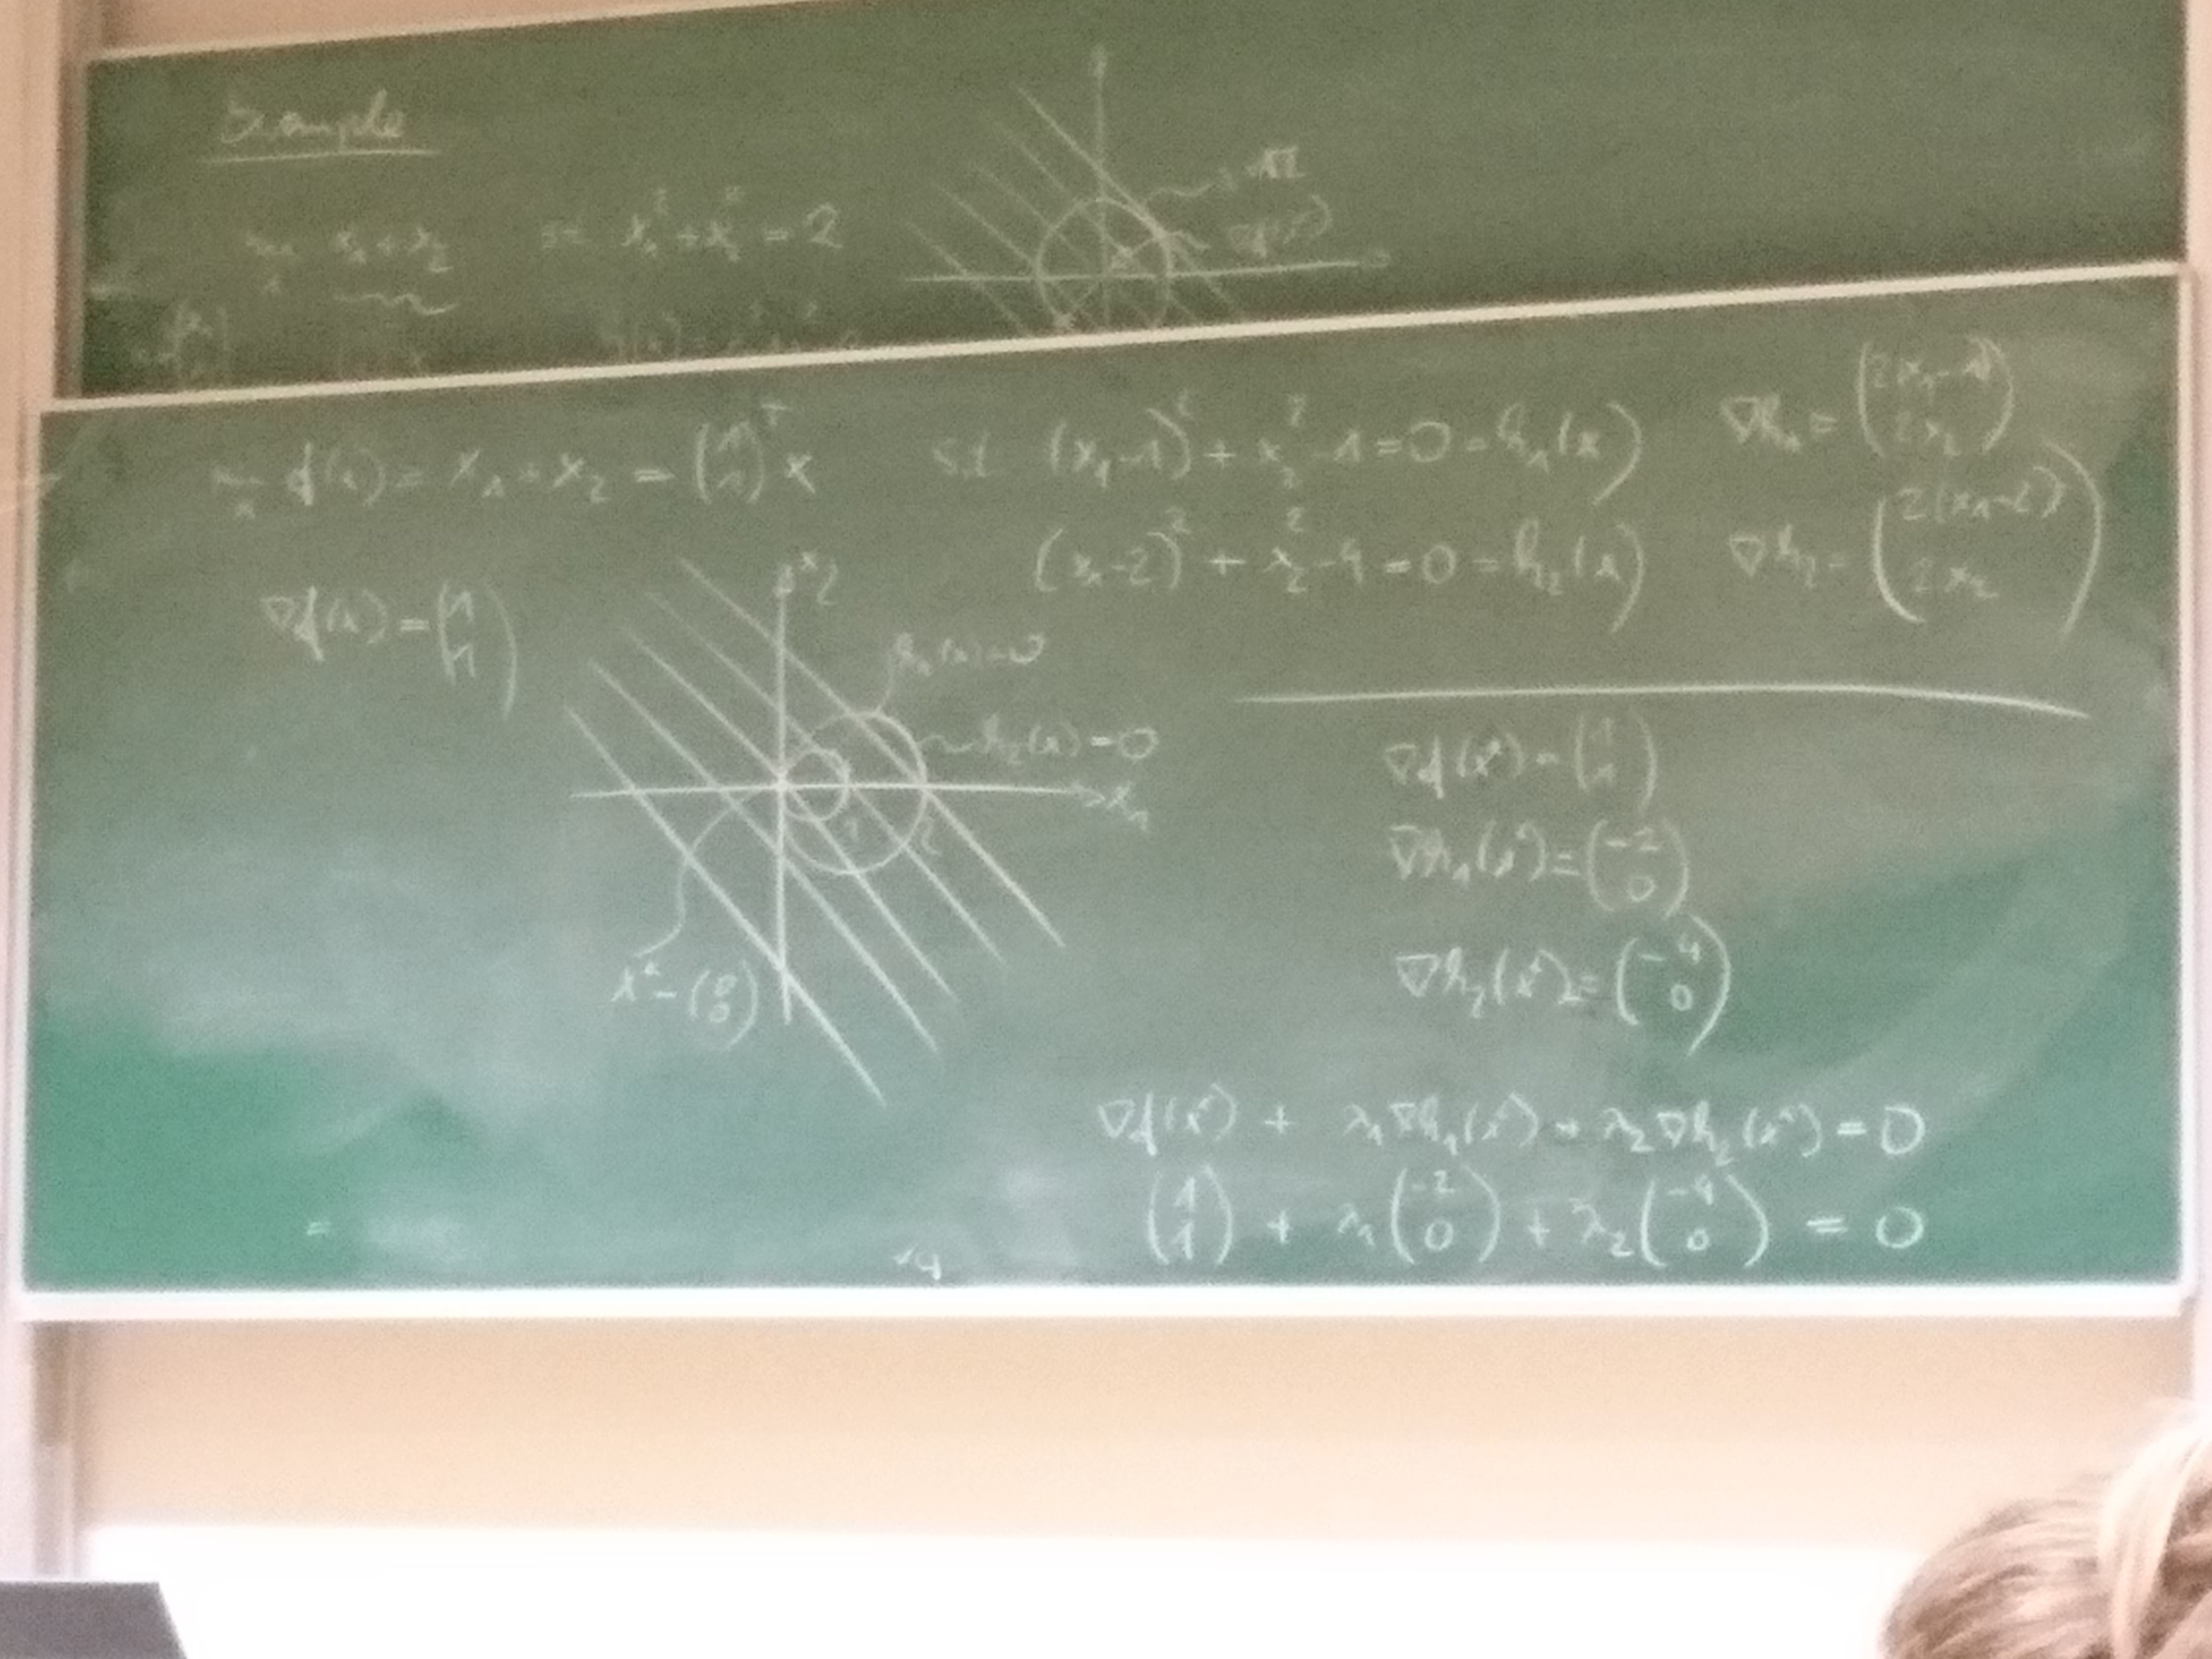
\includegraphics[width=\textwidth]{2017_01_24-ex1.jpg}
\caption{Example1,  24.01.2017\label{fig:ex1}}
\end{figure}

\begin{figure}[H]
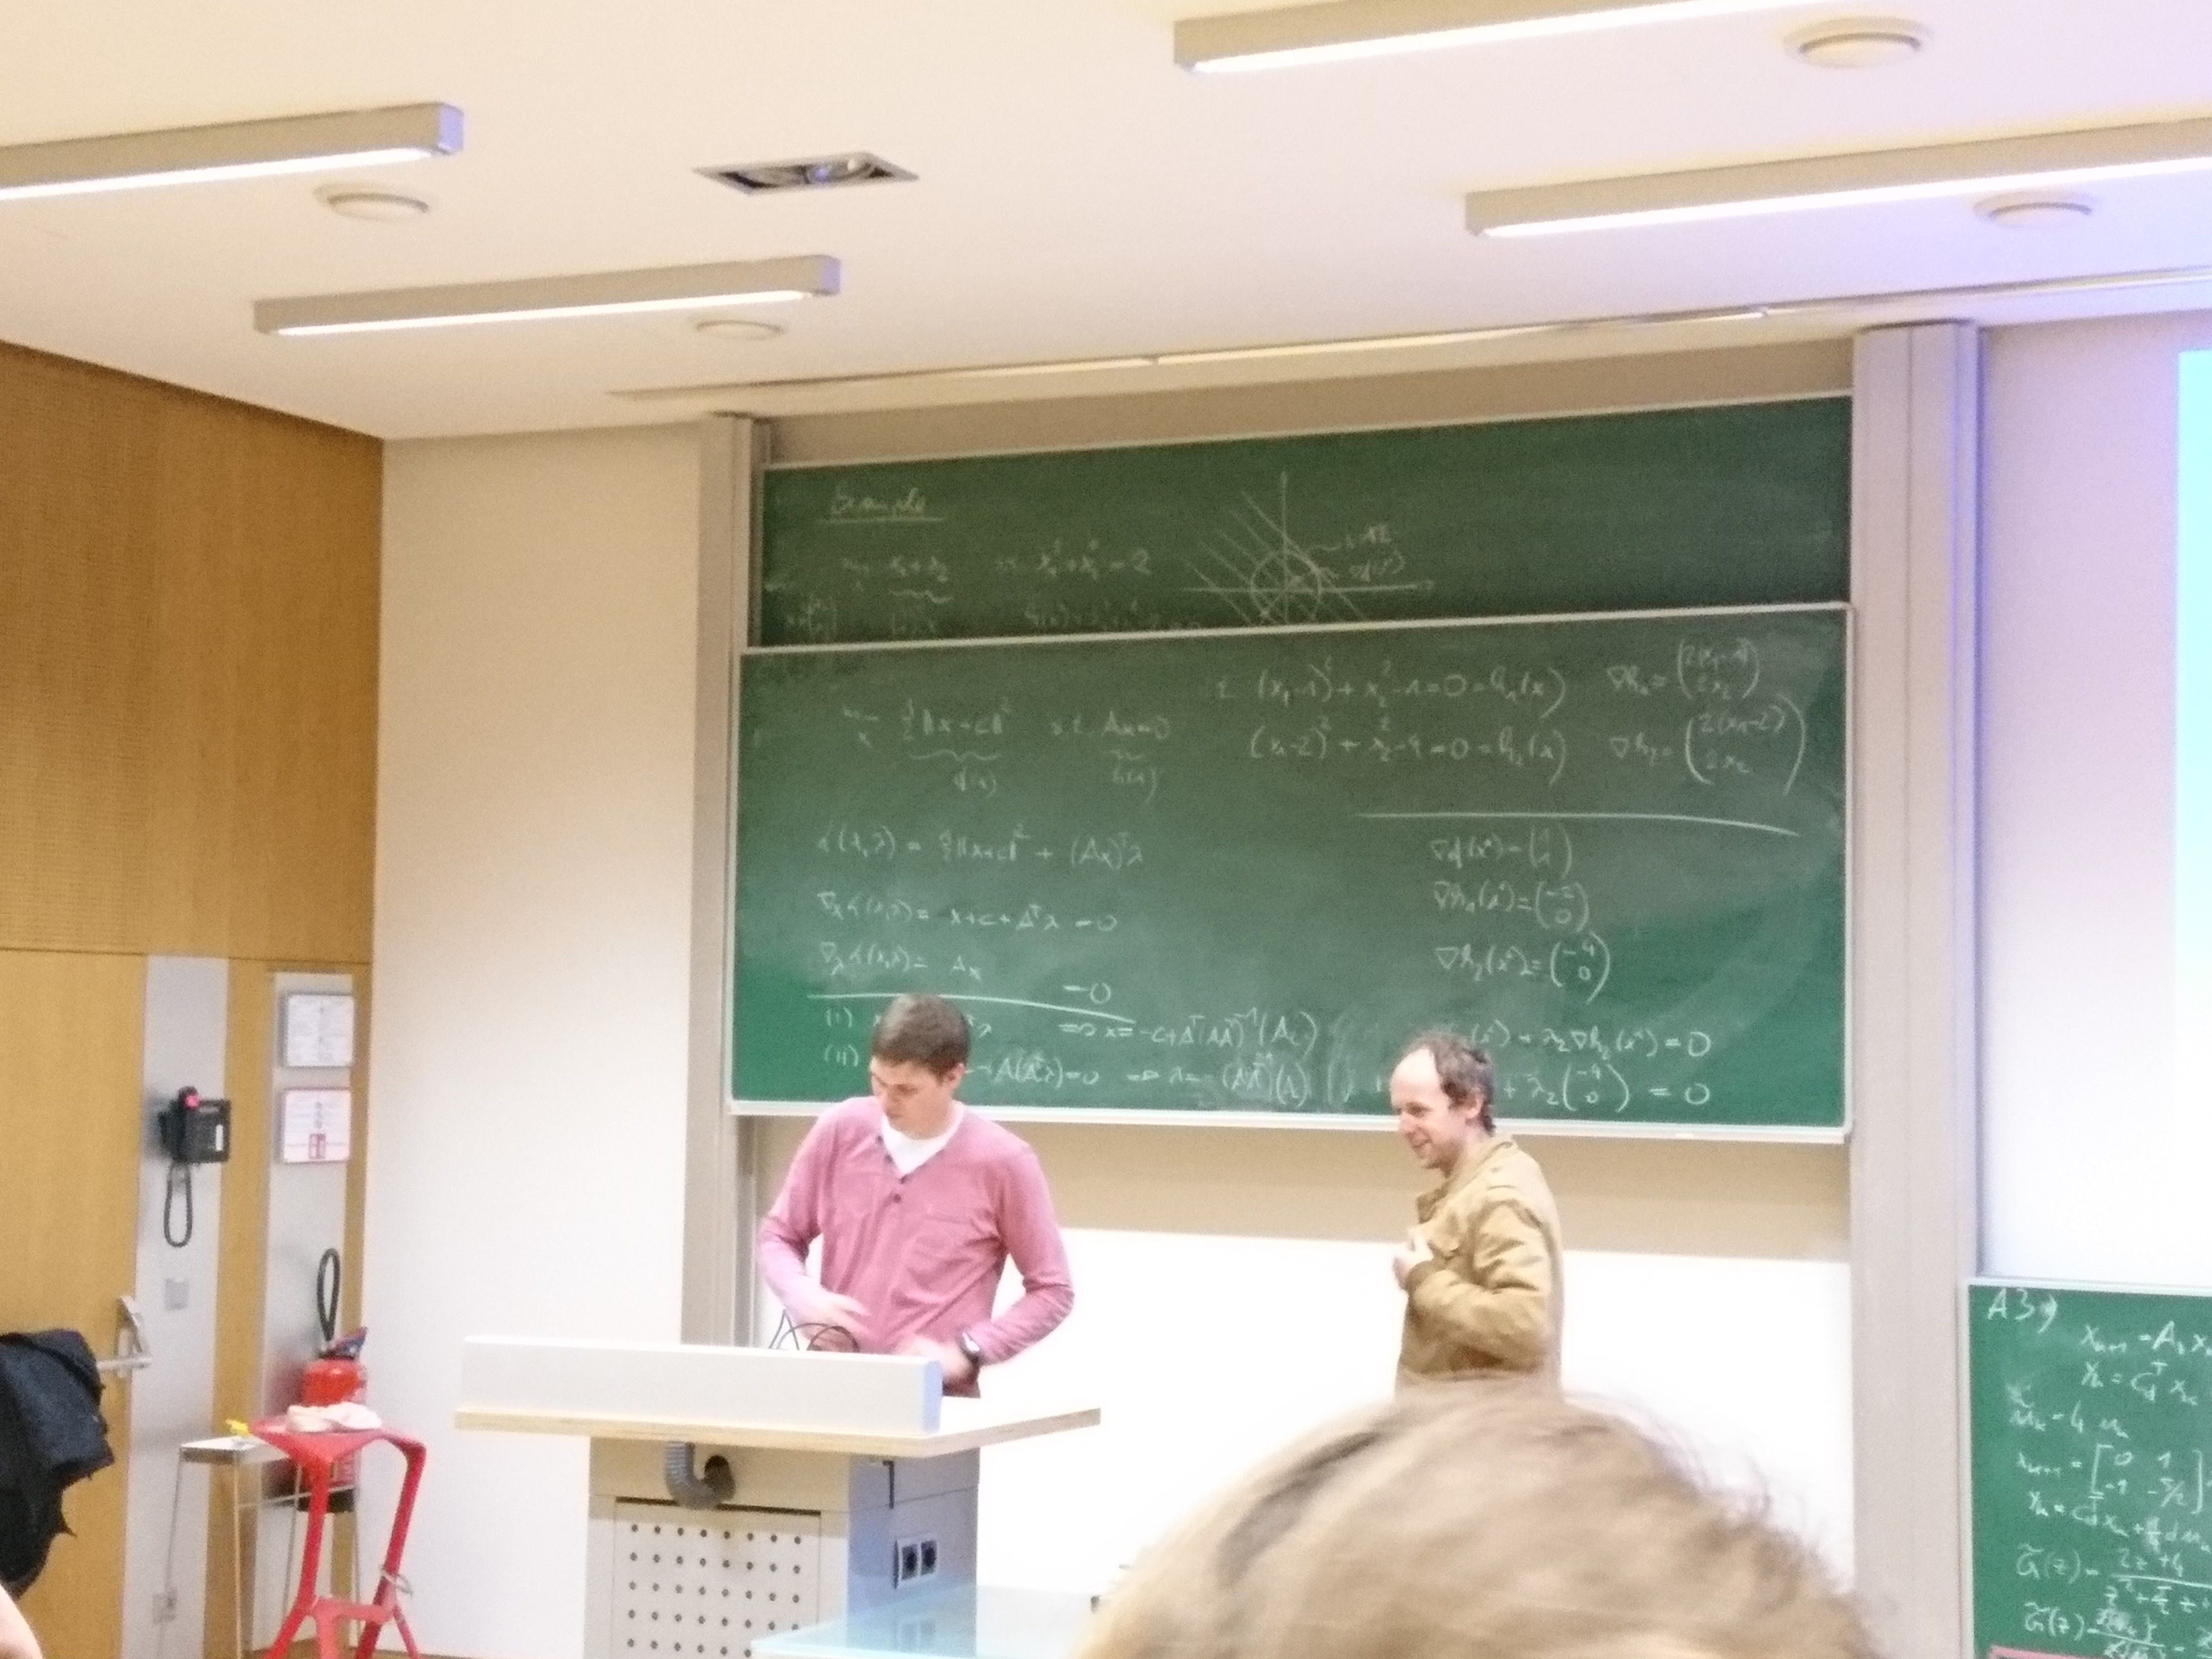
\includegraphics[width=\textwidth]{2017_01_24-ex2.jpg}
\caption{Example 2,  24.01.2017\label{fig:ex2}}
\end{figure}
\end{document}
